%chapter 18

\chapter{Herencia}

La característica del lenguaje más asociada con la programación orientada a objetos es la \textbf{herencia}. La herencia es la capacidad de definir una nueva clase que es una versión modificada de una clase existente. En este capítulo, demostraré la herencia utilizando clases que representan cartas de juego, mazos de cartas y manos de póker.

Si no juegas póker, puedes leer sobre ello en \url{http://en.wikipedia.org/wiki/Poker}, pero no es necesario; te diré lo que necesitas saber para los ejercicios.

Los ejemplos de código de este capítulo están disponibles en \url{https://thinkpython.com/code/Card.py}.

\section{Objetos Carta}

Hay cincuenta y dos cartas en un mazo, cada una de las cuales pertenece a uno de cuatro palos y uno de trece rangos. Los palos son Picas, Corazones, Diamantes y Tréboles (en orden descendente en bridge). Los rangos son As, 2, 3, 4, 5, 6, 7, 8, 9, 10, Jota, Reina y Rey. Dependiendo del juego que estés jugando, un As puede ser más alto que el Rey o más bajo que el 2.

Si queremos definir un nuevo objeto para representar una carta de juego, es obvio cuáles deberían ser los atributos: rango y palo. No es tan obvio qué tipo deberían tener los atributos. Una posibilidad es usar cadenas que contengan palabras como 'Pica' para los palos y 'Reina' para los rangos. Un problema con esta implementación es que no sería fácil comparar cartas para ver cuál tiene un rango o palo más alto.

Una alternativa es usar enteros para \textbf{codificar} los rangos y palos. En este contexto, "codificar" significa que vamos a definir un mapeo entre números y palos, o entre números y rangos. Este tipo de codificación no está destinada a ser un secreto (eso sería "encriptación").

Por ejemplo, esta tabla muestra los palos y los códigos enteros correspondientes:

\begin{center}
\begin{tabular}{|c|c|c|}
\hline
Picas    & $\mapsto$ & 3    \\
Corazones    & $\mapsto$ & 2    \\
Diamantes   & $\mapsto$ & 1    \\
Tréboles    & $\mapsto$ & 0    \\
\hline
\end{tabular}
\end{center}

Este código facilita la comparación de cartas; como los palos más altos se asignan a números más altos, podemos comparar palos comparando sus códigos.

El mapeo para los rangos es bastante obvio; cada uno de los rangos numéricos se asigna al entero correspondiente, y para las cartas con figuras:

\begin{center}
Jota  $\mapsto$  11 \\
Reina  $\mapsto$  12 \\
Rey  $\mapsto$  13 \\
\end{center}

Estoy usando el símbolo $\mapsto$ para dejar claro que estos mapeos no son parte del programa Python. Son parte del diseño del programa, pero no aparecen explícitamente en el código.

La definición de la clase \texttt{Carta} se ve así:

\begin{lstlisting}[language=Python]
class Carta:
    """Representa una carta de juego estándar."""

    def __init__(self, palo=0, rango=2):
        self.palo = palo
        self.rango = rango
\end{lstlisting}

Como es habitual, el método \texttt{\_\_init\_\_} toma un parámetro opcional para cada atributo. La carta predeterminada es el 2 de Tréboles.

Para crear una \texttt{Carta}, llamas a \texttt{Carta} con el palo y rango de la carta que deseas:

\begin{lstlisting}[language=Python]
reina_de_diamantes = Carta(1, 12)
\end{lstlisting}

\section{Atributos de clase}

Para imprimir objetos \texttt{Carta} de una manera que las personas puedan leer fácilmente, necesitamos un mapeo de los códigos enteros a los rangos y palos correspondientes. Una forma natural de hacerlo es con listas de cadenas. Asignamos estas listas a atributos de clase:

\begin{lstlisting}[language=Python]
# dentro de la clase Carta:

nombres_palos = ['Tréboles', 'Diamantes', 'Corazones', 'Picas']
nombres_rangos = [None, 'As', '2', '3', '4', '5', '6', '7', '8', '9', '10', 'Jota', 'Reina', 'Rey']

def __str__(self):
    return '%s de %s' % (Carta.nombres_rangos[self.rango],
                         Carta.nombres_palos[self.palo])
\end{lstlisting}

Variables como \texttt{nombres\_palos} y \texttt{nombres\_rangos}, que se definen dentro de una clase pero fuera de cualquier método, se llaman \textbf{atributos de clase} porque están asociados con el objeto clase \texttt{Carta}.

Este término los distingue de variables como \texttt{palo} y \texttt{rango}, que se llaman \textbf{atributos de instancia} porque están asociados con una instancia particular.

Ambos tipos de atributos se acceden usando notación de punto. Por ejemplo, en \texttt{\_\_str\_\_}, \texttt{self} es un objeto \texttt{Carta}, y \texttt{self.rango} es su rango. De manera similar, \texttt{Carta} es un objeto clase, y \texttt{Carta.nombres\_rangos} es una lista de cadenas asociadas con la clase.

\begin{figure}[h]
\centering
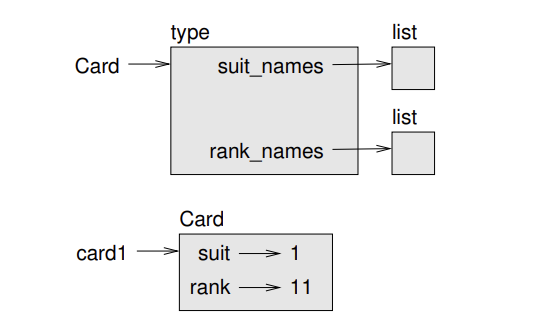
\includegraphics[width=0.5\textwidth]{./images/chapter_18_1.png}
\caption{Diagrama de objeto.}
\label{fig:class_diagrama}
\end{figure}

Cada carta tiene su propio palo y rango, pero solo hay una copia de \texttt{nombres\_palos} y \texttt{nombres\_rangos}.

Juntando todo, la expresión \texttt{Carta.nombres\_rangos[self.rango]} significa "usa el atributo \texttt{rango} del objeto \texttt{self} como un índice en la lista \texttt{nombres\_rangos} de la clase \texttt{Carta}, y selecciona la cadena apropiada."

El primer elemento de \texttt{nombres\_rangos} es \texttt{None} porque no hay una carta con rango cero. Al incluir \texttt{None} como marcador de posición, obtenemos un mapeo con la propiedad agradable de que el índice 2 se asigna a la cadena '2', y así sucesivamente. Para evitar este ajuste, podríamos haber usado un diccionario en lugar de una lista.

Con los métodos que tenemos hasta ahora, podemos crear e imprimir cartas:

\begin{lstlisting}[language=Python]
>>> carta1 = Carta(2, 11)
>>> print(carta1)
Jota de Corazones
\end{lstlisting}

La Figura 18.1 es un diagrama de la clase \texttt{Carta} y una instancia de \texttt{Carta}. \texttt{Carta} es un objeto clase; su tipo es \texttt{type}. \texttt{carta1} es una instancia de \texttt{Carta}, por lo que su tipo es \texttt{Carta}. Para ahorrar espacio, no dibujé el contenido de \texttt{nombres\_palos} y \texttt{nombres\_rangos}.

\section{Comparando cartas}

Para tipos integrados, hay operadores relacionales (<, >, ==, etc.) que comparan valores y determinan cuándo uno es mayor que, menor que o igual a otro. Para tipos definidos por el programador, podemos anular el comportamiento de los operadores integrados proporcionando un método llamado \texttt{\_\_lt\_\_}, que significa "menor que".

\texttt{\_\_lt\_\_} toma dos parámetros, \texttt{self} y \texttt{other}, y devuelve \texttt{True} si \texttt{self} es estrictamente menor que \texttt{other}.

El orden correcto para las cartas no es obvio. Por ejemplo, ¿cuál es mejor, el 3 de Tréboles o el 2 de Diamantes? Uno tiene un rango más alto, pero el otro tiene un palo más alto. Para comparar cartas, tienes que decidir si el rango o el palo es más importante.

La respuesta podría depender del juego que estés jugando, pero para mantener las cosas simples, haremos la elección arbitraria de que el palo es más importante, por lo que todas las Picas superan a todos los Diamantes, y así sucesivamente.

Con eso decidido, podemos escribir \texttt{\_\_lt\_\_}:

\begin{lstlisting}[language=Python]
# dentro de la clase Carta:

def __lt__(self, other):
    # verificar los palos
    if self.palo < other.palo: return True
    if self.palo > other.palo: return False

    # los palos son iguales... verificar los rangos
    return self.rango < other.rango
\end{lstlisting}

Puedes escribir esto de manera más concisa usando comparación de tuplas:

\begin{lstlisting}[language=Python]
# dentro de la clase Carta:

def __lt__(self, other):
    t1 = self.palo, self.rango
    t2 = other.palo, other.rango
    return t1 < t2
\end{lstlisting}

Como ejercicio, escribe un método \texttt{\_\_lt\_\_} para objetos \texttt{Tiempo}. Puedes usar comparación de tuplas, pero también podrías considerar comparar enteros.

\section{Mazos}

Ahora que tenemos \texttt{Cartas}, el siguiente paso es definir \texttt{Mazos}. Como un mazo está compuesto de cartas, es natural que cada \texttt{Mazo} contenga una lista de cartas como atributo.

La siguiente es una definición de clase para \texttt{Mazo}. El método \texttt{\_\_init\_\_} crea el atributo \texttt{cartas} y genera el conjunto estándar de cincuenta y dos cartas:

\begin{lstlisting}[language=Python]
class Mazo:

    def __init__(self):
        self.cartas = []
        for palo in range(4):
            for rango in range(1, 14):
                carta = Carta(palo, rango)
                self.cartas.append(carta)
\end{lstlisting}

La forma más fácil de llenar el mazo es con un bucle anidado. El bucle externo enumera los palos de 0 a 3. El bucle interno enumera los rangos de 1 a 13. Cada iteración crea una nueva \texttt{Carta} con el palo y rango actual, y la agrega a \texttt{self.cartas}.

\section{Imprimiendo el mazo}

Aquí hay un método \texttt{\_\_str\_\_} para \texttt{Mazo}:

\begin{lstlisting}[language=Python]
# dentro de la clase Mazo:

def __str__(self):
    res = []
    for carta in self.cartas:
        res.append(str(carta))
    return '\n'.join(res)
\end{lstlisting}

Este método demuestra una forma eficiente de acumular una cadena larga: construyendo una lista de cadenas y luego usando el método de cadena \texttt{join}. La función integrada \texttt{str} invoca el método \texttt{\_\_str\_\_} en cada carta y devuelve la representación de cadena. Como invocamos \texttt{join} en un carácter de nueva línea, las cartas están separadas por saltos de línea. Así es como se ve el resultado:

\begin{lstlisting}[language=Python]
>>> mazo = Mazo()
>>> print(mazo)
As de Tréboles
2 de Tréboles
3 de Tréboles
...
10 de Picas
Jota de Picas
Reina de Picas
Rey de Picas
\end{lstlisting}

Aunque el resultado aparece en 52 líneas, es una cadena larga que contiene saltos de línea.

\section{Agregar, eliminar, barajar y ordenar}

Para repartir cartas, nos gustaría un método que elimine una carta del mazo y la devuelva. El método \texttt{pop} de lista proporciona una forma conveniente de hacer eso:

\begin{lstlisting}[language=Python]
# dentro de la clase Mazo:
def pop_carta(self):
    return self.cartas.pop()
\end{lstlisting}

Como \texttt{pop} elimina la \textit{última} carta de la lista, estamos repartiendo desde el fondo del mazo. Para agregar una carta, podemos usar el método \texttt{append} de lista:

\begin{lstlisting}[language=Python]
# dentro de la clase Mazo:
def agregar_carta(self, carta):
    self.cartas.append(carta)
\end{lstlisting}

Un método como este que usa otro método sin hacer mucho trabajo a veces se llama \textbf{chapa}. La metáfora proviene de la carpintería, donde una chapa es una capa delgada de madera de buena calidad pegada a la superficie de una pieza más barata para mejorar la apariencia. En este caso, \texttt{agregar\_carta} es un método "delgado" que expresa una operación de lista en términos apropiados para mazos. Mejora la apariencia, o interfaz, de la implementación.

Como otro ejemplo, podemos escribir un método \texttt{barajar} para \texttt{Mazo} usando la función \texttt{shuffle} del módulo \texttt{random}:

\begin{lstlisting}[language=Python]
# dentro de la clase Mazo:
def barajar(self):
    random.shuffle(self.cartas)
\end{lstlisting}

No olvides importar \texttt{random}.

Como ejercicio, escribe un método \texttt{ordenar} para \texttt{Mazo} que use el método \texttt{sort} de lista para ordenar las cartas en un \texttt{Mazo}. \texttt{sort} usa el método \texttt{\_\_lt\_\_} que definimos para determinar el orden.

\section{Herencia}

La herencia es la capacidad de definir una nueva clase que es una versión modificada de una clase existente. Como ejemplo, digamos que queremos una clase para representar una "mano", es decir, las cartas que sostiene un jugador. Una mano es similar a un mazo: ambos están compuestos por una colección de cartas, y ambos requieren operaciones como agregar y eliminar cartas.

Una mano también es diferente de un mazo; hay operaciones que queremos para manos que no tienen sentido para un mazo. Por ejemplo, en póker podríamos comparar dos manos para ver cuál gana. En bridge, podríamos calcular una puntuación para una mano con el fin de hacer una oferta.

Esta relación entre clases—similar, pero diferente—se presta a la herencia. Para definir una nueva clase que herede de una clase existente, pones el nombre de la clase existente entre paréntesis:

\begin{lstlisting}[language=Python]
class Mano(Mazo):
    """Representa una mano de cartas de juego."""
\end{lstlisting}

Esta definición indica que \texttt{Mano} hereda de \texttt{Mazo}; eso significa que podemos usar métodos como \texttt{pop\_carta} y \texttt{agregar\_carta} para \texttt{Manos} así como para \texttt{Mazos}.

Cuando una nueva clase hereda de una existente, la existente se llama \textbf{clase padre} y la nueva clase se llama \textbf{clase hija}.

En este ejemplo, \texttt{Mano} hereda \texttt{\_\_init\_\_} de \texttt{Mazo}, pero no hace exactamente lo que queremos: en lugar de llenar la mano con 52 cartas nuevas, el método \texttt{\_\_init\_\_} para \texttt{Manos} debería inicializar \texttt{cartas} con una lista vacía.

Si proporcionamos un método \texttt{\_\_init\_\_} en la clase \texttt{Mano}, anula el de la clase \texttt{Mazo}:

\begin{lstlisting}[language=Python]
# dentro de la clase Mano:

def __init__(self, etiqueta=''):
    self.cartas = []
    self.etiqueta = etiqueta
\end{lstlisting}

Cuando creas una \texttt{Mano}, Python invoca este método \texttt{\_\_init\_\_}, no el de \texttt{Mazo}.

\begin{lstlisting}[language=Python]
>>> mano = Mano('mano nueva')
>>> mano.cartas
[]
>>> mano.etiqueta
'mano nueva'
\end{lstlisting}

Los otros métodos se heredan de \texttt{Mazo}, por lo que podemos usar \texttt{pop\_carta} y \texttt{agregar\_carta} para repartir una carta:

\begin{lstlisting}[language=Python]
>>> mazo = Mazo()
>>> carta = mazo.pop_carta()
>>> mano.agregar_carta(carta)
>>> print(mano)
Rey de Picas
\end{lstlisting}


Un siguiente paso natural es encapsular este código en un método llamado \texttt{mover\_cartas}:

\begin{lstlisting}[language=Python]
# dentro de la clase Mazo:

def mover_cartas(self, mano, num):
    for i in range(num):
        mano.agregar_carta(self.pop_carta())
\end{lstlisting}

\texttt{mover\_cartas} toma dos argumentos, un objeto \texttt{Mano} y el número de cartas a repartir. Modifica tanto \texttt{self} como \texttt{mano}, y devuelve \texttt{None}.

En algunos juegos, las cartas se mueven de una mano a otra, o de una mano de vuelta al mazo. Puedes usar \texttt{mover\_cartas} para cualquiera de estas operaciones: \texttt{self} puede ser un \texttt{Mazo} o una \texttt{Mano}, y \texttt{mano}, a pesar del nombre, también puede ser un \texttt{Mazo}.

La herencia es una característica útil. Algunos programas que serían repetitivos sin herencia pueden escribirse de manera más elegante con ella. La herencia puede facilitar la reutilización de código, ya que puedes personalizar el comportamiento de las clases padre sin tener que modificarlas. En algunos casos, la estructura de herencia refleja la estructura natural del problema, lo que facilita el diseño.

Por otro lado, la herencia puede hacer que los programas sean difíciles de leer. Cuando se invoca un método, a veces no está claro dónde encontrar su definición. El código relevante puede estar distribuido en varios módulos. Además, muchas de las cosas que se pueden hacer con herencia también se pueden hacer igual o mejor sin ella.

\section{Diagramas de clase}

Hasta ahora hemos visto diagramas de pila, que muestran el estado de un programa, y diagramas de objetos, que muestran los atributos de un objeto y sus valores. Estos diagramas representan una instantánea en la ejecución de un programa, por lo que cambian a medida que el programa se ejecuta.

También son muy detallados; para algunos propósitos, demasiado detallados. Un diagrama de clase es una representación más abstracta de la estructura de un programa. En lugar de mostrar objetos individuales, muestra clases y las relaciones entre ellas.

Hay varios tipos de relaciones entre clases:

\begin{itemize}
    \item Los objetos en una clase pueden contener referencias a objetos en otra clase. Por ejemplo, cada \texttt{Rectángulo} contiene una referencia a un \texttt{Punto}, y cada \texttt{Mazo} contiene referencias a muchas \texttt{Cartas}. Este tipo de relación se llama \textbf{HAS-A}, como en "un Rectángulo tiene un Punto."
    \item Una clase podría heredar de otra. Esta relación se llama \textbf{IS-A}, como en "una Mano es un tipo de Mazo."
    \item Una clase podría depender de otra en el sentido de que los objetos en una clase toman objetos en la segunda clase como parámetros, o usan objetos en la segunda clase como parte de un cálculo. Este tipo de relación se llama \textbf{dependencia}.
\end{itemize}

Un \textbf{diagrama de clase} es una representación gráfica de estas relaciones. Por ejemplo, la Figura 18.2 muestra las relaciones entre \texttt{Carta}, \texttt{Mazo} y \texttt{Mano}.

\begin{figure}[h]
\centering
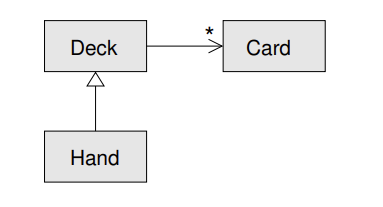
\includegraphics[width=0.5\textwidth]{./images/chapter_18_2.png}
\caption{Diagrama de clase.}
\label{fig:class_diagram}
\end{figure}

La flecha con una cabeza de triángulo hueco representa una relación IS-A; en este caso, indica que \texttt{Mano} hereda de \texttt{Mazo}.

La cabeza de flecha estándar representa una relación HAS-A; en este caso, un \texttt{Mazo} tiene referencias a objetos \texttt{Carta}.

El asterisco (*) cerca de la cabeza de la flecha es una multiplicidad; indica cuántas \texttt{Cartas} tiene un \texttt{Mazo}. Una multiplicidad puede ser un número simple, como 52, un rango, como 5..7, o un asterisco, que indica que un \texttt{Mazo} puede tener cualquier número de \texttt{Cartas}.

No hay dependencias en este diagrama. Normalmente se mostrarían con una flecha discontinua. O si hay muchas dependencias, a veces se omiten.

Un diagrama más detallado podría mostrar que un \texttt{Mazo} en realidad contiene una lista de \texttt{Cartas}, pero los tipos integrados como \texttt{list} y \texttt{dict} generalmente no se incluyen en los diagramas de clase.

\section{Depuración}

La herencia puede dificultar la depuración porque cuando invocas un método en un objeto, puede ser difícil averiguar qué método se invocará.

Supongamos que estás escribiendo una función que funciona con objetos \texttt{Mano}. Te gustaría que funcione con todo tipo de Manos, como \texttt{ManosDePóker}, \texttt{ManosDeBridge}, etc. Si invocas un método como \texttt{barajar}, podrías obtener el definido en \texttt{Mazo}, pero si alguna de las subclases anula este método, obtendrás esa versión en su lugar. Este comportamiento suele ser algo bueno, pero puede ser confuso.

Cada vez que no estés seguro del flujo de ejecución de tu programa, la solución más simple es agregar declaraciones de impresión al principio de los métodos relevantes. Si \texttt{Mazo.barajar} imprime un mensaje que dice algo como "Ejecutando \texttt{Mazo.barajar}", entonces, a medida que el programa se ejecuta, rastreará el flujo de ejecución.

Como alternativa, podrías usar esta función, que toma un objeto y un nombre de método (como una cadena) y devuelve la clase que proporciona la definición del método:

\begin{lstlisting}[language=Python]
def encontrar_clase_definidora(obj, nombre_metodo):
    for ty in type(obj).mro():
        if nombre_metodo in ty.__dict__:
            return ty
\end{lstlisting}

Aquí hay un ejemplo:

\begin{lstlisting}[language=Python]
>>> mano = Mano()
>>> encontrar_clase_definidora(mano, 'barajar')
<class '__main__.Mazo'>
\end{lstlisting}

Así que el método \texttt{barajar} para esta \texttt{Mano} es el de \texttt{Mazo}.

\texttt{encontrar\_clase\_definidora} usa el método \texttt{mro} para obtener la lista de objetos de clase (tipos) que se buscarán para los métodos. "MRO" significa "orden de resolución de método", que es la secuencia de clases que Python busca para "resolver" un nombre de método.

Aquí hay una sugerencia de diseño: cuando anulas un método, la interfaz del nuevo método debe ser la misma que la del antiguo. Debe tomar los mismos parámetros, devolver el mismo tipo y obedecer las mismas precondiciones y poscondiciones. Si sigues esta regla, encontrarás que cualquier función diseñada para trabajar con una instancia de una clase padre, como un \texttt{Mazo}, también funcionará con instancias de clases hijas como \texttt{Mano} y \texttt{ManoDePóker}.

Si violas esta regla, que se llama el "principio de sustitución de Liskov", tu código colapsará como (lo siento) un castillo de naipes.

\section{Encapsulamiento de datos}

Los capítulos anteriores demuestran un plan de desarrollo que podríamos llamar "diseño orientado a objetos". Identificamos los objetos que necesitábamos—como \texttt{Punto}, \texttt{Rectángulo} y \texttt{Tiempo}—y definimos clases para representarlos. En cada caso, hay una correspondencia obvia entre el objeto y alguna entidad en el mundo real (o al menos un mundo matemático).

Pero a veces es menos obvio qué objetos necesitas y cómo deberían interactuar. En ese caso, necesitas un plan de desarrollo diferente. De la misma manera que descubrimos interfaces de funciones mediante encapsulamiento y generalización, podemos descubrir interfaces de clases mediante \textbf{encapsulamiento de datos}.

El análisis de Markov, de la Sección 13.8, proporciona un buen ejemplo. Si descargas mi código de \url{https://thinkpython.com/code/markov.py}, verás que usa dos variables globales—\texttt{mapa\_sufijos} y \texttt{prefijo}—que se leen y escriben desde varias funciones.

\begin{lstlisting}[language=Python]
mapa_sufijos = {}
prefijo = ()
\end{lstlisting}

Debido a que estas variables son globales, solo podemos ejecutar un análisis a la vez. Si leemos dos textos, sus prefijos y sufijos se agregarían a las mismas estructuras de datos (lo que genera algunos textos generados interesantes).

Para ejecutar múltiples análisis y mantenerlos separados, podemos encapsular el estado de cada análisis en un objeto. Así es como se ve:

\begin{lstlisting}[language=Python]
class Markov:
    def __init__(self):
        self.mapa_sufijos = {}
        self.prefijo = ()
\end{lstlisting}

A continuación, transformamos las funciones en métodos. Por ejemplo, aquí está \texttt{procesar\_palabra}:

\begin{lstlisting}[language=Python]
def procesar_palabra(self, palabra, orden=2):
    if len(self.prefijo) < orden:
        self.prefijo += (palabra,)
        return

    try:
        self.mapa_sufijos[self.prefijo].append(palabra)
    except KeyError:
        # si no hay entrada para este prefijo, haz una
        self.mapa_sufijos[self.prefijo] = [palabra]
    self.prefijo = desplazar(self.prefijo, palabra)
\end{lstlisting}

Transformar un programa como este—cambiar el diseño sin cambiar el comportamiento—es otro ejemplo de refactorización (ver Sección 4.7).

Este ejemplo sugiere un plan de desarrollo para diseñar objetos y métodos:

\begin{enumerate}
    \item Comienza escribiendo funciones que lean y escriban variables globales (cuando sea necesario).
    \item Una vez que el programa funcione, busca asociaciones entre variables globales y las funciones que las usan.
    \item Encapsula las variables relacionadas como atributos de un objeto.
    \item Transforma las funciones asociadas en métodos de la nueva clase.
\end{enumerate}

Como ejercicio, descarga mi código Markov de \url{https://thinkpython.com/code/markov.py}, y sigue los pasos descritos anteriormente para encapsular las variables globales como atributos de una nueva clase llamada \texttt{Markov}. Solución: \url{https://thinkpython.com/code/markov2.py}.

\section{Glosario}

\begin{description}
    \item[codificar:] Representar un conjunto de valores usando otro conjunto de valores construyendo un mapeo entre ellos.
    \item[atributo de clase:] Un atributo asociado con un objeto de clase. Los atributos de clase se definen dentro de una definición de clase pero fuera de cualquier método.
    \item[atributo de instancia:] Un atributo asociado con una instancia de una clase.
    \item[chapa:] Un método o función que proporciona una interfaz diferente a otra función sin hacer mucho cálculo.
    \item[herencia:] La capacidad de definir una nueva clase que es una versión modificada de una clase previamente definida.
    \item[clase padre:] La clase desde la cual una clase hija hereda.
    \item[clase hija:] Una nueva clase creada heredando de una clase existente; también llamada "subclase".
    \item[relación IS-A:] Una relación entre una clase hija y su clase padre.
    \item[relación HAS-A:] Una relación entre dos clases donde las instancias de una clase contienen referencias a instancias de la otra.
    \item[dependencia:] Una relación entre dos clases donde las instancias de una clase usan instancias de la otra clase, pero no las almacenan como atributos.
    \item[diagrama de clase:] Un diagrama que muestra las clases en un programa y las relaciones entre ellas.
    \item[multiplicidad:] Una notación en un diagrama de clase que muestra, para una relación HAS-A, cuántas referencias hay a instancias de otra clase.
    \item[encapsulamiento de datos:] Un plan de desarrollo de programas que implica un prototipo que usa variables globales y una versión final que convierte las variables globales en atributos de instancia.
\end{description}

\section{Ejercicios}

\textbf{Ejercicio 18.1.} Para el siguiente programa, dibuja un diagrama de clases UML que muestre estas clases y las relaciones entre ellas.

\begin{lstlisting}[language=Python]
class PadrePingPong:
    pass

class Ping(PadrePingPong):
    def __init__(self, pong):
        self.pong = pong

class Pong(PadrePingPong):
    def __init__(self, pings=None):
        if pings is None:
            self.pings = []
        else:
            self.pings = pings

    def agregar_ping(self, ping):
        self.pings.append(ping)

pong = Pong()
ping = Ping(pong)
pong.agregar_ping(ping)
\end{lstlisting}

\textbf{Ejercicio 18.2.} Escribe un método de \texttt{Mazo} llamado \texttt{repartir\_manos} que tome dos parámetros, el número de manos y el número de cartas por mano. Debe crear el número apropiado de objetos \texttt{Mano}, repartir el número apropiado de cartas por mano y devolver una lista de \texttt{Manos}.

\textbf{Ejercicio 18.3.} Las siguientes son las posibles manos en póker, en orden creciente de valor y decreciente de probabilidad:

\begin{itemize}
    \item par: dos cartas con el mismo rango
    \item doble par: dos pares de cartas con el mismo rango
    \item tercia: tres cartas con el mismo rango
    \item escalera: cinco cartas con rangos en secuencia (los Ases pueden ser altos o bajos, por lo que As-2-3-4-5 es una escalera y también 10-Jota-Reina-Rey-As, pero Reina-Rey-As-2-3 no lo es)
    \item color: cinco cartas con el mismo palo
    \item full house: tres cartas con un rango, dos cartas con otro
    \item poker: cuatro cartas con el mismo rango
    \item escalera de color: cinco cartas en secuencia (como se definió anteriormente) y con el mismo palo
\end{itemize}

El objetivo de estos ejercicios es estimar la probabilidad de sacar estas varias manos.

\begin{enumerate}
    \item Descarga los siguientes archivos de \url{https://thinkpython.com/code}:
    \begin{itemize}
        \item \texttt{Card.py}: Una versión completa de las clases \texttt{Carta}, \texttt{Mazo} y \texttt{Mano} en este capítulo.
        \item \texttt{PokerHand.py}: Una implementación incompleta de una clase que representa una mano de póker, y algo de código que la prueba.
    \end{itemize}
    \item Si ejecutas \texttt{PokerHand.py}, reparte siete manos de póker de 7 cartas y verifica si alguna de ellas contiene un color. Lee este código cuidadosamente antes de continuar.
    \item Agrega métodos a \texttt{PokerHand.py} llamados \texttt{tiene\_par}, \texttt{tiene\_doble\_par}, etc. que devuelvan \texttt{True} o \texttt{False} según si la mano cumple o no con los criterios relevantes. Tu código debería funcionar correctamente para "manos" que contengan cualquier número de cartas (aunque 5 y 7 son los tamaños más comunes).
    \item Escribe un método llamado \texttt{clasificar} que determine la clasificación de mayor valor para una mano y establezca el atributo \texttt{etiqueta} en consecuencia. Por ejemplo, una mano de 7 cartas podría contener un color y un par; debería etiquetarse como "color".
    \item Cuando estés convencido de que tus métodos de clasificación funcionan, el siguiente paso es estimar las probabilidades de las varias manos. Escribe una función en \texttt{PokerHand.py} que baraje un mazo de cartas, lo divida en manos, clasifique las manos y cuente el número de veces que aparecen varias clasificaciones.
    \item Imprime una tabla de las clasificaciones y sus probabilidades. Ejecuta tu programa con números cada vez mayores de manos hasta que los valores de salida converjan a un grado razonable de precisión. Compara tus resultados con los valores en \url{http://en.wikipedia.org/wiki/Hand_rankings}.
\end{enumerate}

Solución: \url{https://thinkpython.com/code/PokerHandSoln.py}.